
\documentclass{article}

% Required packages
\usepackage{amssymb}
\usepackage{amsmath}
\usepackage{graphicx}
\usepackage{geometry}
\usepackage{tikz}
\usepackage{array}
\usepackage{booktabs}
\usepackage{enumitem}
\usepackage{listings}
\usepackage{xcolor}
\usepackage{fancyhdr}
\usepackage{float}
\usepackage{subcaption}

% Set page geometry
\geometry{a4paper, margin=1in}

% Configure listings for Python
\lstset{
  language=Python,
  basicstyle=\ttfamily\footnotesize,
  numbers=left,
  numberstyle=\tiny\color{gray},
  frame=single,
  breaklines=true,
  breakatwhitespace=true,
  captionpos=b,
  tabsize=4,
  showspaces=false,
  showstringspaces=false,
  showtabs=false,
  commentstyle=\color{gray}\textit,
  keywordstyle=\color{blue}\bfseries,
  stringstyle=\color{red}
}

\begin{document}

\pagestyle{fancy}
\chead{DSC 255: Machine Learning Fundamentals (Spring 2025)}
\lhead{Homework 6}
\rhead{Randall Rogers}

\subsection*{Solution 1}
\noindent\rule{\textwidth}{0.4pt}\\

\subsubsection*{Step 1}
\parbox{\textwidth}{
We are given the prediction rule is defined as:
} 

$$\left(2 x_{1}-x_{2}-6\right)$$

To find the decision boundary we set the prediction rule equal to zero:
$$2 x_{1}-x_{2}-6 = 0 \hspace{1cm} \text{or} \hspace{1cm} x_{2} = 2 x_{1} - 6$$

We can rearrange this to express $x_2$ in terms of $x_1$:
$$x_{2} = 2 x_{1} - 6$$

\subsubsection*{Step 2}
\parbox{\textwidth}{
Find the point $(x_{1},x_{2})$ where the decision boundary intersects the $x_{1}$ axis (i.e. $x_{2}=0$):

$$x_{2} = 2 x_{1} - 6 \hspace{0.2cm} \rightarrow \hspace{0.2cm} 0 = 2 x_{1} - 6 \hspace{0.2cm} \rightarrow \hspace{0.2cm} 2 x_{1} = 6 \hspace{0.2cm} \rightarrow \hspace{0.2cm} x_{1} = 3$$

Hence, the decision boundary intersects the $x_{1}$ axis at $(3,0)$
}
\subsubsection*{Step 3}
\parbox{\textwidth}{
Find the point $(x_{1},x_{2})$ where the decision boundary intersects the $x_{2}$ axis (i.e. $x_{1}=0$):

$$x_{2} = 2 x_{1} - 6 \hspace{0.2cm} \rightarrow \hspace{0.2cm} x_{2} = 2 (0) - 6 \hspace{0.2cm} \rightarrow \hspace{0.2cm} 2 x_{2} = -6 $$

Hence, the decision boundary intersects the $x_{1}$ axis at $(0,6)$
}

\subsubsection*{Step 4}
\parbox{\textwidth}{
Test prediction rule at the point $(0,0)$ to determine the classification above the decision boundary.

$$2 x_{1} - x_{2} - 6 \hspace{0.2cm} \rightarrow \hspace{0.2cm}  2(0) - 0 - 6 \hspace{0.2cm} \rightarrow \hspace{0.2cm} -6$$

It follows that, $2 x_{1} - x_{2} - 6 < 0$  at $(0,0)$ and this area above the decision boundary will be classified as negative. 

}

\subsubsection*{Step 5}
\parbox{\textwidth}{
Visualize the decision boundary:
}

\begin{center}
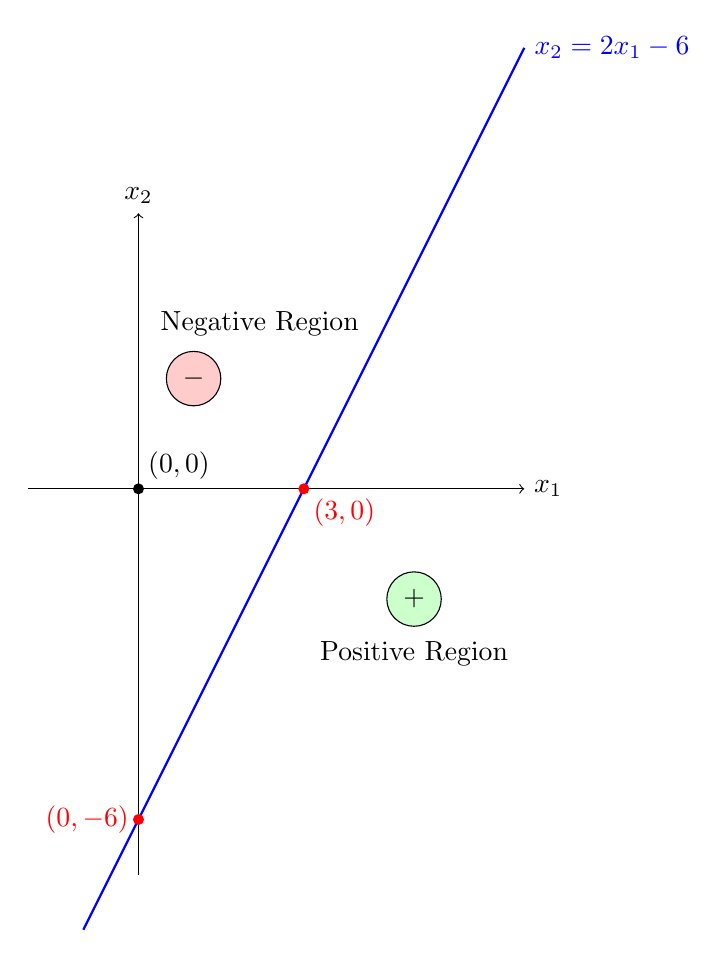
\begin{tikzpicture}[scale=0.7]
    % Draw axes
    \draw[->] (-2,0) -- (7,0) node[right] {$x_1$};
    \draw[->] (0,-7) -- (0,5) node[above] {$x_2$};
    
    % Draw decision boundary
    \draw[blue, thick] (-1,-8) -- (7,8) node[right] {$x_2 = 2x_1 - 6$};
    
    % Mark intersections
    \fill[red] (3,0) circle (0.1) node[below right] {$(3,0)$};
    \fill[red] (0,-6) circle (0.1) node[left] {$(0,-6)$};
    
    % Label regions
    \node at (5,-3) {Positive Region};
    \node at (2.2,3) {Negative Region};
    
    % Add + and - symbols to make it clearer
    \node[circle, draw, fill=green!20] at (5,-2) {$+$};
    \node[circle, draw, fill=red!20] at (1,2) {$-$};
    
    % Origin
    \fill[black] (0,0) circle (0.1) node[above right] {$(0,0)$};
\end{tikzpicture}
\end{center}

\subsubsection*{\normalfont}{$\therefore$ The decision boundary is the line $x_2 = 2x_1 - 6$, which intersects the $x_{1}$ axis at $(3,0)$ and the  $x_{2}$ axis at $(0,-6)$. The region below this line is classified as positive, and the region above it is classified as negative.}

\noindent\rule{\textwidth}{0.4pt}\\

\newpage

\subsection*{Solution 2 (a)}
\noindent\rule{\textwidth}{0.4pt}

\subsubsection*{\normalfont}{$\therefore$ The statement: \textit{The data set is linearly separable.} is \textbf{definitely true}. The Perceptron algorithm will convergethe data is linearly separable and we are given: \textit{it converges after making k updates}.}

\noindent\rule{\textwidth}{0.4pt}\\

\subsection*{Solution 2 (b)}
\noindent\rule{\textwidth}{0.4pt}\\

\subsubsection*{\normalfont}{$\therefore$ The statement: \textit{If the process were repeated with a different random permutation, it would again converge} is \textbf{definitely true}. Since the Perceptron algorithm will converge regardless of order.}

\noindent\rule{\textwidth}{0.4pt}\\

\subsection*{Solution 2 (c)}
\noindent\rule{\textwidth}{0.4pt}\\

\subsubsection*{\normalfont}{$\therefore$ The statement: \textit{If the process were repeated with a different random permutation, it would again converge after making k updates} is \textbf{possibly false}. The number of updates required for convergence can change depending on the order of data.}

\noindent\rule{\textwidth}{0.4pt}\\

\subsection*{Solution 2 (d)}
\noindent\rule{\textwidth}{0.4pt}\\

\subsubsection*{\normalfont}{$\therefore$ The statement: \textit{k is at most n} is \textbf{possibly false}. The number of updates $k$ can exceed the number of data points $n$.}

\noindent\rule{\textwidth}{0.4pt}\\

\newpage

\subsection*{Solution 3}
\noindent\rule{\textwidth}{0.4pt}\\

\subsubsection*{Step 1}
\parbox{\textwidth}{
A point $(x, y)$ is misclassified when:

$$y(w \cdot x + b) \leq 0 $$

The Perceptron algorithm tells us to update $w$ and $b$ when a point is misclassified as the following:
$$ w= w +yx \hspace{0.2cm} \text{and} \hspace{0.2cm} b = b + y$$

}

\subsubsection*{Step 2}
\parbox{\textwidth}{
We are given the following: 
\begin{itemize}
    \item Perceptron algorithm performs $p+q$ updates before converging
    \item $p$ updates on data points with label $y_i = -1$
    \item $q$ updates on data points with label $y_i = +1$
\end{itemize}

}

\subsubsection*{Step 3}
\parbox{\textwidth}{
Let the initial bias be $b = 0$. Each time a misclassified point is encountered, the bias is updated by adding the label $y_i$.

\begin{itemize}
    \item For each of the $p$ negative examples ($y_i = -1$), the bias decreases by $1$: total change is $-p$
    \item For each of the $q$ positive examples ($y_i = 1$), the bias increases by $1$: total change is $q$
\end{itemize}
}

\subsubsection*{\normalfont}{$\therefore$ The final value of the parameter $b$ is $q - p$.}

\noindent\rule{\textwidth}{0.4pt}\\

\newpage

\subsection*{Solution 4 (a)}
\noindent\rule{\textwidth}{0.4pt}\\

\subsubsection*{Step 1}
\parbox{\textwidth}{
Given:
\begin{itemize}
    \item SVM classifier in $\mathbb{R}^{2}$
    \item Weight vector $w = (3, 4)$
    \item Bias term $b = -12$
\end{itemize}

The prediction rule would then be defined as:

$$\left(3x_{1}+4x_{2}-12\right)$$

} 

\subsubsection*{Step 2}
\parbox{\textwidth}{
Find the point $(x_{1},x_{2})$ where the decision boundary intersects the $x_{1}$ axis (i.e. $x_{2}=0$):

$$3x_1 + 4(0) - 12 = 0 \hspace{0.2cm} \rightarrow \hspace{0.2cm} 3x_1 = 12 \hspace{0.2cm} \rightarrow \hspace{0.2cm} x_1 = 4$$

Hence, the decision boundary intersects the $x_{1}$ axis at $(4,0)$
}

\subsubsection*{Step 3}
\parbox{\textwidth}{
Find the point $(x_{1},x_{2})$ where the decision boundary intersects the $x_{2}$ axis (i.e. $x_{1}=0$):

$$3(0) + 4x_2 - 12 = 0 \hspace{0.2cm} \rightarrow \hspace{0.2cm} 4x_2 = 12 \hspace{0.2cm} \rightarrow \hspace{0.2cm} x_2 = 3$$

Hence, the decision boundary intersects the $x_{2}$ axis at $(0,3)$
}

\subsubsection*{Step 4}
\parbox{\textwidth}{
Test prediction rule at the point $(0,0)$ to determine the classification below the decision boundary.

$$3(0) + 4(0) - 12 = -12$$

It follows that $3x_1 + 4x_2 - 12 < 0$ at $(0,0)$, and so this region below the decision boundary will be classified as negative.
}

\subsubsection*{Step 5}
\parbox{\textwidth}{
Visualize the decision boundary:
}

\begin{center}
\begin{tikzpicture}[scale=0.7]
    % Draw axes
    \draw[->] (-2,0) -- (7,0) node[right] {$x_1$};
    \draw[->] (0,-2) -- (0,5) node[above] {$x_2$};
    
    % Draw decision boundary
    \draw[blue, thick] (0,3) -- (4,0) node at (6,2.5) {$3x_1 + 4x_2 = 12$: Decision Boundary};
    
    % Mark intersections
    \fill[red] (4,0) circle (0.1) node[below right] {$(4,0)$};
    \fill[red] (0,3) circle (0.1) node[left] {$(0,3)$};
    
    
    % Origin
    %\fill[black] (0,0) circle (0.1) node[above right] {$(0,0)$};
\end{tikzpicture}
\end{center}

\noindent\rule{\textwidth}{0.4pt}\\

\newpage

\subsection*{Solution 4 (b)}
\noindent\rule{\textwidth}{0.4pt}\\

\subsubsection*{Step 1}
\parbox{\textwidth}{
The margin boundaries are defined as:
\begin{align}
w \cdot x + b &= 1 \quad \text{(positive margin boundary)}\\
w \cdot x + b &= -1 \quad \text{(negative margin boundary)}
\end{align}

Remember the prediction rule would then is defined as:

$$\left(3x_{1}+4x_{2}-12\right)$$
}

\subsubsection*{Step 2}
\parbox{\textwidth}{
Solve for right hand boundary ($\left(3x_{1}+4x_{2}-13\right)$):

Find the point $(x_{1},x_{2})$ where the right hand boundary intersects the $x_{1}$ axis (i.e. $x_{2}=0$):

$$3x_{1} + 4(0) - 13 = 0 \hspace{0.2cm} \rightarrow \hspace{0.2cm} 3x_{1} = 13 \hspace{0.2cm} \rightarrow \hspace{0.2cm} x_{1} = \frac{13}{3}$$

Hence, the right hand boundary intersects the $x_{1}$ axis at $\left(\frac{13}{3}, 0\right)$.\\


Now, find the point $(x_{1},x_{2})$ where the right hand boundary intersects the $x_{2}$ axis (i.e. $x_{1}=0$):

$$3(0) + 4x_{2} - 13 = 0 \hspace{0.2cm} \rightarrow \hspace{0.2cm} 4x_{2} = 13 \hspace{0.2cm} \rightarrow \hspace{0.2cm} x_{2} = \frac{13}{4}$$

Hence, the right hand boundary intersects the $x_{2}$ axis at $\left(0, \frac{13}{4}\right)$.
}

\subsubsection*{Step 3}
\parbox{\textwidth}{
Solve for left hand boundary ($\left(3x_{1}+4x_{2}-11\right)$):

Find the point $(x_{1},x_{2})$ where the left hand boundary intersects the $x_{1}$ axis (i.e. $x_{2}=0$):

$$3x_{1} + 4(0) - 11 = 0 \hspace{0.2cm} \rightarrow \hspace{0.2cm} 3x_{1} = 11 \hspace{0.2cm} \rightarrow \hspace{0.2cm} x_{1} = \frac{11}{3}$$

Hence, the left hand boundary intersects the $x_{1}$ axis at $\left(\frac{11}{3}, 0\right)$.\\

Now, find the point $(x_{1},x_{2})$ where the left hand boundary intersects the $x_{2}$ axis (i.e. $x_{1}=0$):

$$3(0) + 4x_{2} - 11 = 0 \hspace{0.2cm} \rightarrow \hspace{0.2cm} 4x_{2} = 11 \hspace{0.2cm} \rightarrow \hspace{0.2cm} x_{2} = \frac{11}{4}$$

Hence, the left hand boundary intersects the $x_{2}$ axis at $\left(0, \frac{11}{4}\right)$.
}

\subsubsection*{Step 4}
\parbox{\textwidth}{
Visualize the left hand and right hand boundaries:
}

\begin{center}
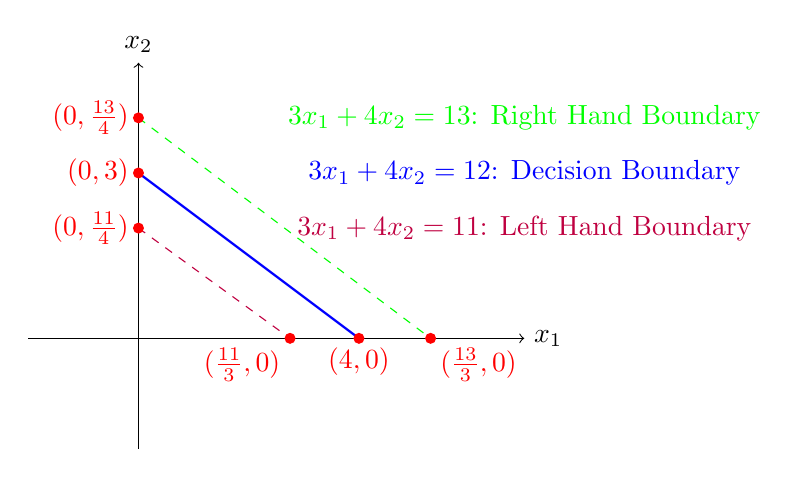
\begin{tikzpicture}[scale=0.7]
    % Draw axes
    \draw[->] (-2,0) -- (7,0) node[right] {$x_1$};
    \draw[->] (0,-2) -- (0,5) node[above] {$x_2$};
    
    % Draw decision boundary
    \draw[green, dashed] (0,4) -- (5.3,0) node at (7,4) {$3x_1 + 4x_2 = 13$: Right Hand Boundary};
    \draw[purple, dashed] (0,2) -- (2.75,0) node at (7,2) {$3x_1 + 4x_2 = 11$: Left Hand Boundary};
    \draw[blue, thick] (0,3) -- (4,0) node at (7,3) {$3x_1 + 4x_2 = 12$: Decision Boundary};
    % Mark intersections
    \fill[red] (5.3,0) circle (0.1) node[below right] {$(\frac{13}{3},0)$};
    \fill[red] (0,4) circle (0.1) node[left] {$(0,\frac{13}{4})$};
    \fill[red] (2.75,0) circle (0.1) node[below left] {$(\frac{11}{3},0)$};
    \fill[red] (0,2) circle (0.1) node[left] {$(0,\frac{11}{4})$};
    \fill[red] (4,0) circle (0.1) node[below] {$(4,0)$};
    \fill[red] (0,3) circle (0.1) node[left] {$(0,3)$};
    
    
    % Origin
    %\fill[black] (0,0) circle (0.1) node[above right] {$(0,0)$};
\end{tikzpicture}
\end{center}

\noindent\rule{\textwidth}{0.4pt}\\

\newpage

\subsection*{Solution 4 (c)}
\noindent\rule{\textwidth}{0.4pt}\\

\subsubsection*{Step 1}
\parbox{\textwidth}{
The margin of an SVM classifier is defined below where $||w||$, the Euclidean norm of the weight vector:
$$\text{Margin} = \frac{2}{||w||} = \frac{2}{\sqrt{w_1^2 + w_2^2}}$$
}

\subsubsection*{Step 2}
\parbox{\textwidth}{
Calculate the margin:
\begin{align*}
\text{Margin} &= \frac{2}{||w||}\\
&= \frac{2}{\sqrt{3^2 + 4^2}}\\
&= \frac{2}{\sqrt{25}}\\
&= \frac{2}{5}\\
&= 0.4
\end{align*}
}

\subsubsection*{\normalfont}{$\therefore$ The margin of this SVM classifier is $\frac{2}{5}$ or  $0.4$ units.}

\noindent\rule{\textwidth}{0.4pt}\\

\newpage

\subsection*{Solution 4 (d)}
\noindent\rule{\textwidth}{0.4pt}\\

\subsubsection*{Step 1}
\parbox{\textwidth}{
Use visulization from \textbf{Solution 4 (a)} and plot the point $(2,2)$:
}

\begin{center}
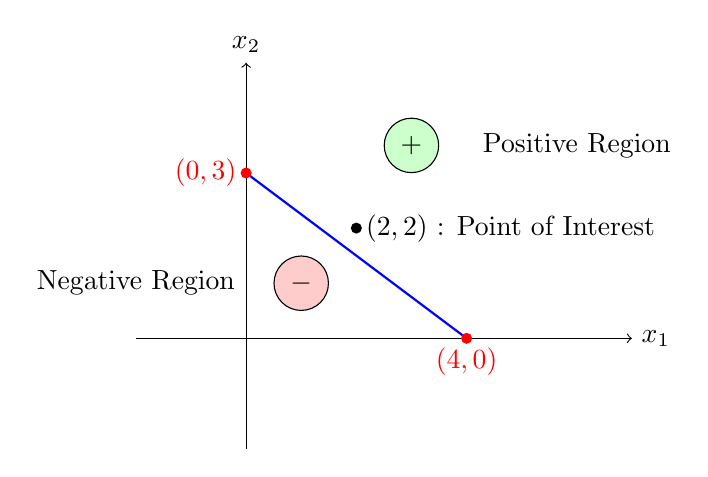
\begin{tikzpicture}[scale=0.7]
    % Draw axes
    \draw[->] (-2,0) -- (7,0) node[right] {$x_1$};
    \draw[->] (0,-2) -- (0,5) node[above] {$x_2$};
    
    % Draw decision boundary

    \draw[blue, thick] (0,3) -- (4,0);
    % Mark intersections

    \fill[red] (4,0) circle (0.1) node[below] {$(4,0)$};
    \fill[red] (0,3) circle (0.1) node[left] {$(0,3)$};
    \fill[black] (2,2) circle (0.1) node[right] {$(2,2)$ : Point of Interest};

    % Label regions
    \node at (6,3.5) {Positive Region};
    \node at (-2,1) {Negative Region};
    
    % Add + and - symbols to make it clearer
    \node[circle, draw, fill=green!20] at (3,3.5) {$+$};
    \node[circle, draw, fill=red!20] at (1,1) {$-$};
    
    
    % Origin
    %\fill[black] (0,0) circle (0.1) node[above right] {$(0,0)$};
\end{tikzpicture}
\end{center}

\subsubsection*{\normalfont}{$\therefore$ The point $(2, 2)$ would be classified as positive.}

\noindent\rule{\textwidth}{0.4pt}\\

\newpage

\subsection*{Solution 5 (a)}
\noindent\rule{\textwidth}{0.4pt}\\

\subsubsection*{Step 1}
\parbox{\textwidth}{
In a soft-margin SVM, the support vectors are the data points that:
\begin{itemize}
    \item Lie exactly on the margin boundaries (slack variable $\xi_i = 0$)
    \item Lie between the margin boundary and the decision boundary (slack variable $0 < \xi_i < 1$)
    \item Lie on the wrong side of the margin boundary (slack variable $\xi_i \geq 1$)
\end{itemize}

The slack variable $\xi_i$ represents the degree of misclassification for each point. It measures how far a point is from its correct margin boundary.
}

\subsubsection*{Step 2}
\parbox{\textwidth}{
Let's identify the support vectors in the given figure:

\begin{center}
  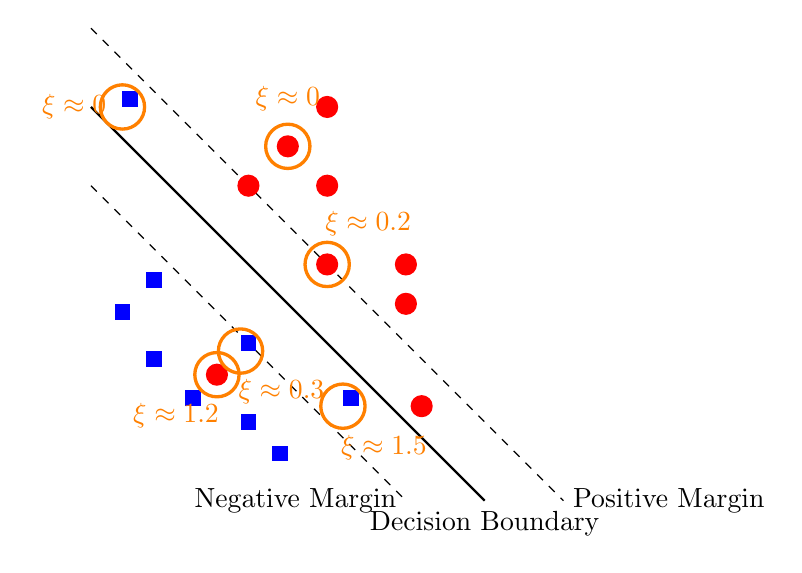
\begin{tikzpicture}
  % Solid decision boundary (approx. average of lines)
  \draw[thick] (0,5) -- (5,0) node[below] {Decision Boundary};
  \draw[dashed] (0,6) -- (6,0) node[right] {Positive Margin};
  \draw[dashed] (0,4) -- (4,0) node[left] {Negative Margin};

  % Blue squares (negative class)
  \foreach \x/\y in {0.7/2.7,0.7/1.7, 0.3/2.3,1.2/1.2,1.9/0.9,2.3/0.5 ,1.9/1.9, 3.2/1.2, 0.4/5.0} {
    \fill[blue] (\x,\y) rectangle ++(0.2,0.2);}

  % Red circles (positive class)
  \foreach \x/\y in {1.6/1.6, 4.2/1.2, 2/4, 3/3,3/4,3/5,2.5/4.5, 4/3,4/2.5} {
    \fill[red] (\x,\y) circle (4pt);}
    
  % Highlight support vectors and add slack variable values
  % Support vectors on or near margin boundaries (ξ = 0)
  \draw[orange, very thick, circle] (0.4,5.0) circle (8pt) node[left] {$\xi \approx 0$};
  \draw[orange, very thick, circle] (2.5,4.5) circle (8pt) node[above] {$\xi \approx 0$};
  
  % Support vectors between margin and decision boundary (0 < ξ < 1)
  \draw[orange, very thick, circle] (1.9,1.9) circle (8pt) node[below right] {$\xi \approx 0.3$};
  \draw[orange, very thick, circle] (3,3) circle (8pt) node[above right] {$\xi \approx 0.2$};
  
  % Support vectors on wrong side of margin (ξ ≥ 1)
  \draw[orange, very thick, circle] (1.6,1.6) circle (8pt) node[below left] {$\xi \approx 1.2$};
  \draw[orange, very thick, circle] (3.2,1.2) circle (8pt) node[below right] {$\xi \approx 1.5$};
  
  \end{tikzpicture}
\end{center}
}

\subsubsection*{Step 3}
\parbox{\textwidth}{
Let's explain the identified support vectors:

\begin{enumerate}
    \item \textbf{Support vectors with $\xi \approx 0$:}
    \begin{itemize}
        \item The blue square at approximately $(0.4, 5.0)$ lies very close to the negative margin boundary.
        \item The red circle at approximately $(2.5, 4.5)$ lies very close to the positive margin boundary.
        \item These points have slack variables close to zero because they are almost exactly on their respective margin boundaries.
    \end{itemize}
    
    \item \textbf{Support vectors with $0 < \xi < 1$:}
    \begin{itemize}
        \item The blue square at approximately $(1.9, 1.9)$ is between the negative margin and the decision boundary.
        \item The red circle at approximately $(3, 3)$ is between the positive margin and the decision boundary.
        \item These points have slack variables between 0 and 1 because they are inside the margin but on the correct side of the decision boundary.
    \end{itemize}
    
    \item \textbf{Support vectors with $\xi \geq 1$:}
    \begin{itemize}
        \item The red circle at approximately $(1.6, 1.6)$ is on the wrong side of the decision boundary.
        \item The blue square at approximately $(3.2, 1.2)$ is also on the wrong side of the decision boundary.
        \item These points have slack variables greater than or equal to 1 because they are misclassified by the decision boundary.
    \end{itemize}
\end{enumerate}
}

\subsubsection*{\normalfont}{$\therefore$ The support vectors are the points circled in orange in the figure above, with their approximate slack variable values indicated. Support vectors include points exactly on the margin boundaries ($\xi \approx 0$), points between the margin and decision boundary ($0 < \xi < 1$), and misclassified points ($\xi \geq 1$).}

\noindent\rule{\textwidth}{0.4pt}\\

\newpage

\subsection*{Solution 5 (b)}
\noindent\rule{\textwidth}{0.4pt}\\

\subsubsection*{Step 1}
\parbox{\textwidth}{
Recall the optimization problem for soft-margin SVM:

$$\min_{w, b, \xi} \frac{1}{2} ||w||^2 + C \sum_{i=1}^{n} \xi_i$$

subject to:
$$y_i(w \cdot x_i + b) \geq 1 - \xi_i, \quad \xi_i \geq 0 \quad \forall i$$

The parameter $C$ controls the trade-off between maximizing the margin (minimizing $||w||^2$) and minimizing the classification error (minimizing $\sum \xi_i$).
}

\subsubsection*{Step 2}
\parbox{\textwidth}{
When $C$ is increased:
\begin{itemize}
    \item The penalty for misclassification and margin violations becomes higher.
    \item The optimization will prioritize reducing the slack variables $\xi_i$ over maximizing the margin.
    \item This means the model will try harder to correctly classify all training points, potentially at the expense of a smaller margin.
\end{itemize}
}

\subsubsection*{Step 3}
\parbox{\textwidth}{
Let's compare the effects of different values of $C$:

\begin{center}
\begin{tabular}{|c|c|c|}
\hline
\textbf{Small $C$} & \textbf{Medium $C$} & \textbf{Large $C$} \\
\hline
Larger margin & Balanced trade-off & Smaller margin \\
More misclassifications & Some misclassifications & Fewer misclassifications \\
Underfitting risk & Good generalization & Overfitting risk \\
\hline
\end{tabular}
\end{center}

In our specific example, increasing $C$ would likely:
\begin{itemize}
    \item Make the decision boundary adjust to reduce the misclassifications (the red circle at $(1.6, 1.6)$ and the blue square at $(3.2, 1.2)$).
    \item Potentially reduce the margin between the dashed lines to better accommodate the training points.
\end{itemize}
}

\begin{center}
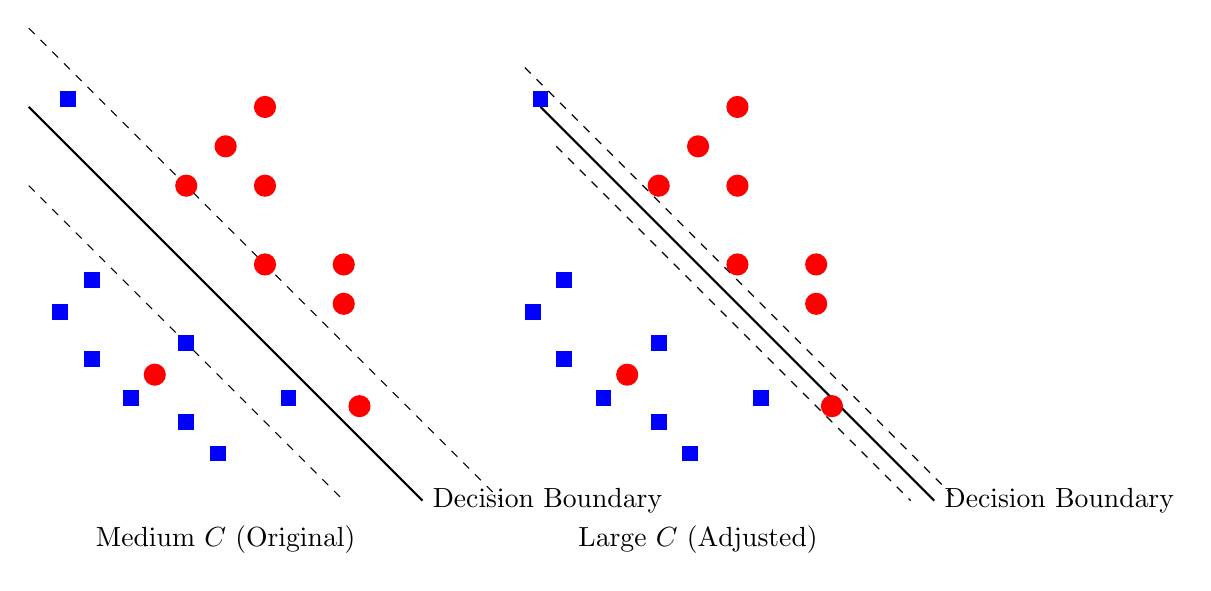
\begin{tikzpicture}
% Original SVM (medium C)
\begin{scope}[xshift=-3cm]
  \draw[thick] (0,5) -- (5,0) node[right] {Decision Boundary};
  \draw[dashed] (0,6) -- (6,0);
  \draw[dashed] (0,4) -- (4,0);
  
  % Blue squares
  \foreach \x/\y in {0.7/2.7,0.7/1.7, 0.3/2.3,1.2/1.2,1.9/0.9,2.3/0.5 ,1.9/1.9, 3.2/1.2, 0.4/5.0} {
    \fill[blue] (\x,\y) rectangle ++(0.2,0.2);}

  % Red circles
  \foreach \x/\y in {1.6/1.6, 4.2/1.2, 2/4, 3/3,3/4,3/5,2.5/4.5, 4/3,4/2.5} {
    \fill[red] (\x,\y) circle (4pt);}
    
  \node at (2.5,-0.5) {Medium $C$ (Original)};
\end{scope}

% Large C SVM
\begin{scope}[xshift=3cm]
  % Adjusted decision boundary for larger C
  \draw[thick] (0.5,5) -- (5.5,0) node[right] {Decision Boundary};
  \draw[dashed] (0.3,5.5) -- (5.8,0);
  \draw[dashed] (0.7,4.5) -- (5.2,0);
  
  % Blue squares
  \foreach \x/\y in {0.7/2.7,0.7/1.7, 0.3/2.3,1.2/1.2,1.9/0.9,2.3/0.5 ,1.9/1.9, 3.2/1.2, 0.4/5.0} {
    \fill[blue] (\x,\y) rectangle ++(0.2,0.2);}

  % Red circles
  \foreach \x/\y in {1.6/1.6, 4.2/1.2, 2/4, 3/3,3/4,3/5,2.5/4.5, 4/3,4/2.5} {
    \fill[red] (\x,\y) circle (4pt);}
    
  \node at (2.5,-0.5) {Large $C$ (Adjusted)};
\end{scope}
\end{tikzpicture}
\end{center}

\subsubsection*{\normalfont}{$\therefore$ If the factor $C$ in the soft-margin SVM optimization problem were increased, we would expect the margin to \textbf{decrease}. This is because a larger $C$ places more emphasis on correctly classifying all training points, even if it means having a smaller margin.}

\noindent\rule{\textwidth}{0.4pt}\\

\newpage

\subsection*{Solution 6 (a)}
\noindent\rule{\textwidth}{0.4pt}\\

\subsubsection*{Step 1}
\parbox{\textwidth}{
Let's recall the dual form of the Perceptron algorithm:

In the dual form, we represent the weight vector $w$ as a linear combination of the training examples:
$$w = \sum_{i=1}^{n} \alpha_i y_i x_i$$

where $\alpha_i$ counts how many times example $i$ has been misclassified during training.
}

\subsubsection*{Step 2}
\parbox{\textwidth}{
In the standard Perceptron algorithm, when a point $(x_i, y_i)$ is misclassified, we update:
$$w \leftarrow w + y_i x_i$$

In the dual form, this corresponds to incrementing $\alpha_i$ by 1:
$$\alpha_i \leftarrow \alpha_i + 1$$

Initially, all $\alpha_i$ values are set to 0. Each time a point is misclassified, its corresponding $\alpha_i$ is incremented by 1.
}

\subsubsection*{Step 3}
\parbox{\textwidth}{
Since the algorithm performs $k$ updates in total, and each update increments exactly one $\alpha_i$ by 1, we know that:

\begin{itemize}
    \item Each $\alpha_i$ represents the number of times example $i$ was misclassified
    \item Each $\alpha_i$ must be a non-negative integer
    \item Some examples might never be misclassified, so their $\alpha_i$ remains 0
    \item Some examples might be misclassified multiple times, so their $\alpha_i$ could be greater than 1
\end{itemize}
}

\subsubsection*{\normalfont}{$\therefore$ The statement "Each $\alpha_i$ is either 0 or 1" is \textbf{possibly false}. While some $\alpha_i$ values may be 0 (never misclassified) or 1 (misclassified once), it's possible for an example to be misclassified multiple times during training, resulting in $\alpha_i > 1$.}

\noindent\rule{\textwidth}{0.4pt}\\

\newpage

\subsection*{Solution 6 (b)}
\noindent\rule{\textwidth}{0.4pt}\\

\subsubsection*{Step 1}
\parbox{\textwidth}{
We know that the Perceptron algorithm makes a total of $k$ updates, and each update corresponds to incrementing exactly one $\alpha_i$ by 1.
}

\subsubsection*{Step 2}
\parbox{\textwidth}{
Initially, all $\alpha_i$ values are set to 0. After $k$ updates, each incrementing one $\alpha_i$ by 1, the sum of all $\alpha_i$ values must be equal to $k$:

$$\sum_{i=1}^{n} \alpha_i = k$$

This is because each update contributes exactly 1 to the sum of $\alpha_i$ values, and there are $k$ updates in total.
}

\subsubsection*{\normalfont}{$\therefore$ The statement "$\sum_{i} \alpha_i = k$" is \textbf{necessarily true}. Since each of the $k$ updates increments exactly one $\alpha_i$ by 1, and all $\alpha_i$ values start at 0, the sum of all $\alpha_i$ values must equal $k$.}

\noindent\rule{\textwidth}{0.4pt}\\

\newpage

\subsection*{Solution 6 (c)}
\noindent\rule{\textwidth}{0.4pt}\\

\subsubsection*{Step 1}
\parbox{\textwidth}{
We need to determine the maximum number of nonzero coordinates in the vector $\alpha$.
}

\subsubsection*{Step 2}
\parbox{\textwidth}{
A coordinate $\alpha_i$ is nonzero if and only if the corresponding example $(x_i, y_i)$ has been misclassified at least once during training.

In the worst case, each of the $k$ updates could be applied to a different example, resulting in $k$ different examples having their $\alpha_i$ incremented to 1.

However, it's also possible that some examples are misclassified multiple times, which would result in fewer than $k$ nonzero coordinates in $\alpha$.
}

\subsubsection*{Step 3}
\parbox{\textwidth}{
Let's consider a simple example to illustrate:

Suppose we have 5 training examples and the algorithm makes $k = 3$ updates:
\begin{itemize}
    \item If the updates are applied to examples 1, 2, and 3, then $\alpha = (1, 1, 1, 0, 0)$ with 3 nonzero coordinates.
    \item If the updates are applied to examples 1, 1, and 2, then $\alpha = (2, 1, 0, 0, 0)$ with 2 nonzero coordinates.
\end{itemize}

In general, the number of nonzero coordinates in $\alpha$ is at most $k$ (when each update is applied to a different example) and at least 1 (when all updates are applied to the same example).
}

\subsubsection*{\normalfont}{$\therefore$ The statement "$\alpha$ has at most $k$ nonzero coordinates" is \textbf{necessarily true}. Since there are $k$ updates in total, at most $k$ different examples can be misclassified, resulting in at most $k$ nonzero $\alpha_i$ values.}

\noindent\rule{\textwidth}{0.4pt}\\

\newpage

\subsection*{Solution 6 (d)}
\noindent\rule{\textwidth}{0.4pt}\\

\subsubsection*{Step 1}
\parbox{\textwidth}{
We need to determine whether the convergence of the Perceptron algorithm implies that the training data is linearly separable.
}

\subsubsection*{Step 2}
\parbox{\textwidth}{
Recall the Perceptron Convergence Theorem: If the training data is linearly separable, then the Perceptron algorithm will converge in a finite number of updates.

The converse is also true: If the Perceptron algorithm converges, then the training data must be linearly separable. This is because:

\begin{itemize}
    \item Convergence means the algorithm has found a weight vector $w$ and bias $b$ such that all training examples are correctly classified.
    \item This means there exists a hyperplane defined by $w \cdot x + b = 0$ that separates the positive and negative examples.
    \item By definition, this makes the data linearly separable.
\end{itemize}
}

\subsubsection*{Step 3}
\parbox{\textwidth}{
It's important to note that if the data is not linearly separable, the Perceptron algorithm will never converge - it will continue to make updates indefinitely as it cycles through the data.

Since we're told that the algorithm converges after $k$ updates, this implies that the algorithm has found a separating hyperplane, which means the data must be linearly separable.
}

\subsubsection*{\normalfont}{$\therefore$ The statement "The training data must be linearly separable" is \textbf{necessarily true}. The convergence of the Perceptron algorithm implies that it has found a hyperplane that correctly classifies all training examples, which by definition means the data is linearly separable.}

\noindent\rule{\textwidth}{0.4pt}\\

\newpage
\begin{center}
  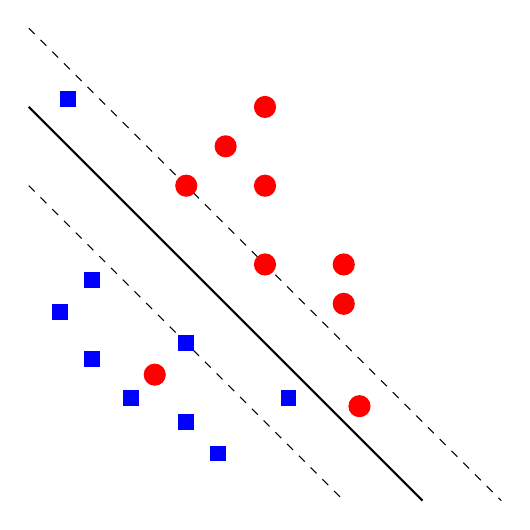
\begin{tikzpicture}
  % Solid decision boundary (approx. average of lines)
  \draw[thick] (0,5) -- (5,0);
  \draw[dashed] (0,6) -- (6,0);
  \draw[dashed] (0,4) -- (4,0);

  % Blue squares
  \foreach \x/\y in {0.7/2.7,0.7/1.7, 0.3/2.3,1.2/1.2,1.9/0.9,2.3/0.5 ,1.9/1.9, 3.2/1.2, 0.4/5.0} {
    \fill[blue] (\x,\y) rectangle ++(0.2,0.2);}

  % Red circles
  \foreach \x/\y in {1.6/1.6, 4.2/1.2, 2/4, 3/3,3/4,3/5,2.5/4.5, 4/3,4/2.5} {
    \fill[red] (\x,\y) circle (4pt);}
  \end{tikzpicture}
\end{center}

\end{document}
